Key steps to be taken for manned missions to Mars for the proposed design are:
\begin{itemize}
\item Crew module design and decelerator detailed design
\item Ground and unmanned flight testing to further design and component \gls{trl}
\item Production and integration
\item Crew preparation and training
\item Establishing infrastructure on Mars
\end{itemize}

\subsubsection{Project Gantt chart}
Having finished this preliminary investigation, careful consideration is required on the planning of the rest of the design, production and operation phases. A Gantt chart of the steps following this preliminary investigation is presented in Figure \ref{fig:projectganttchart}.\\

\begin{figure}[h]
	\centering
	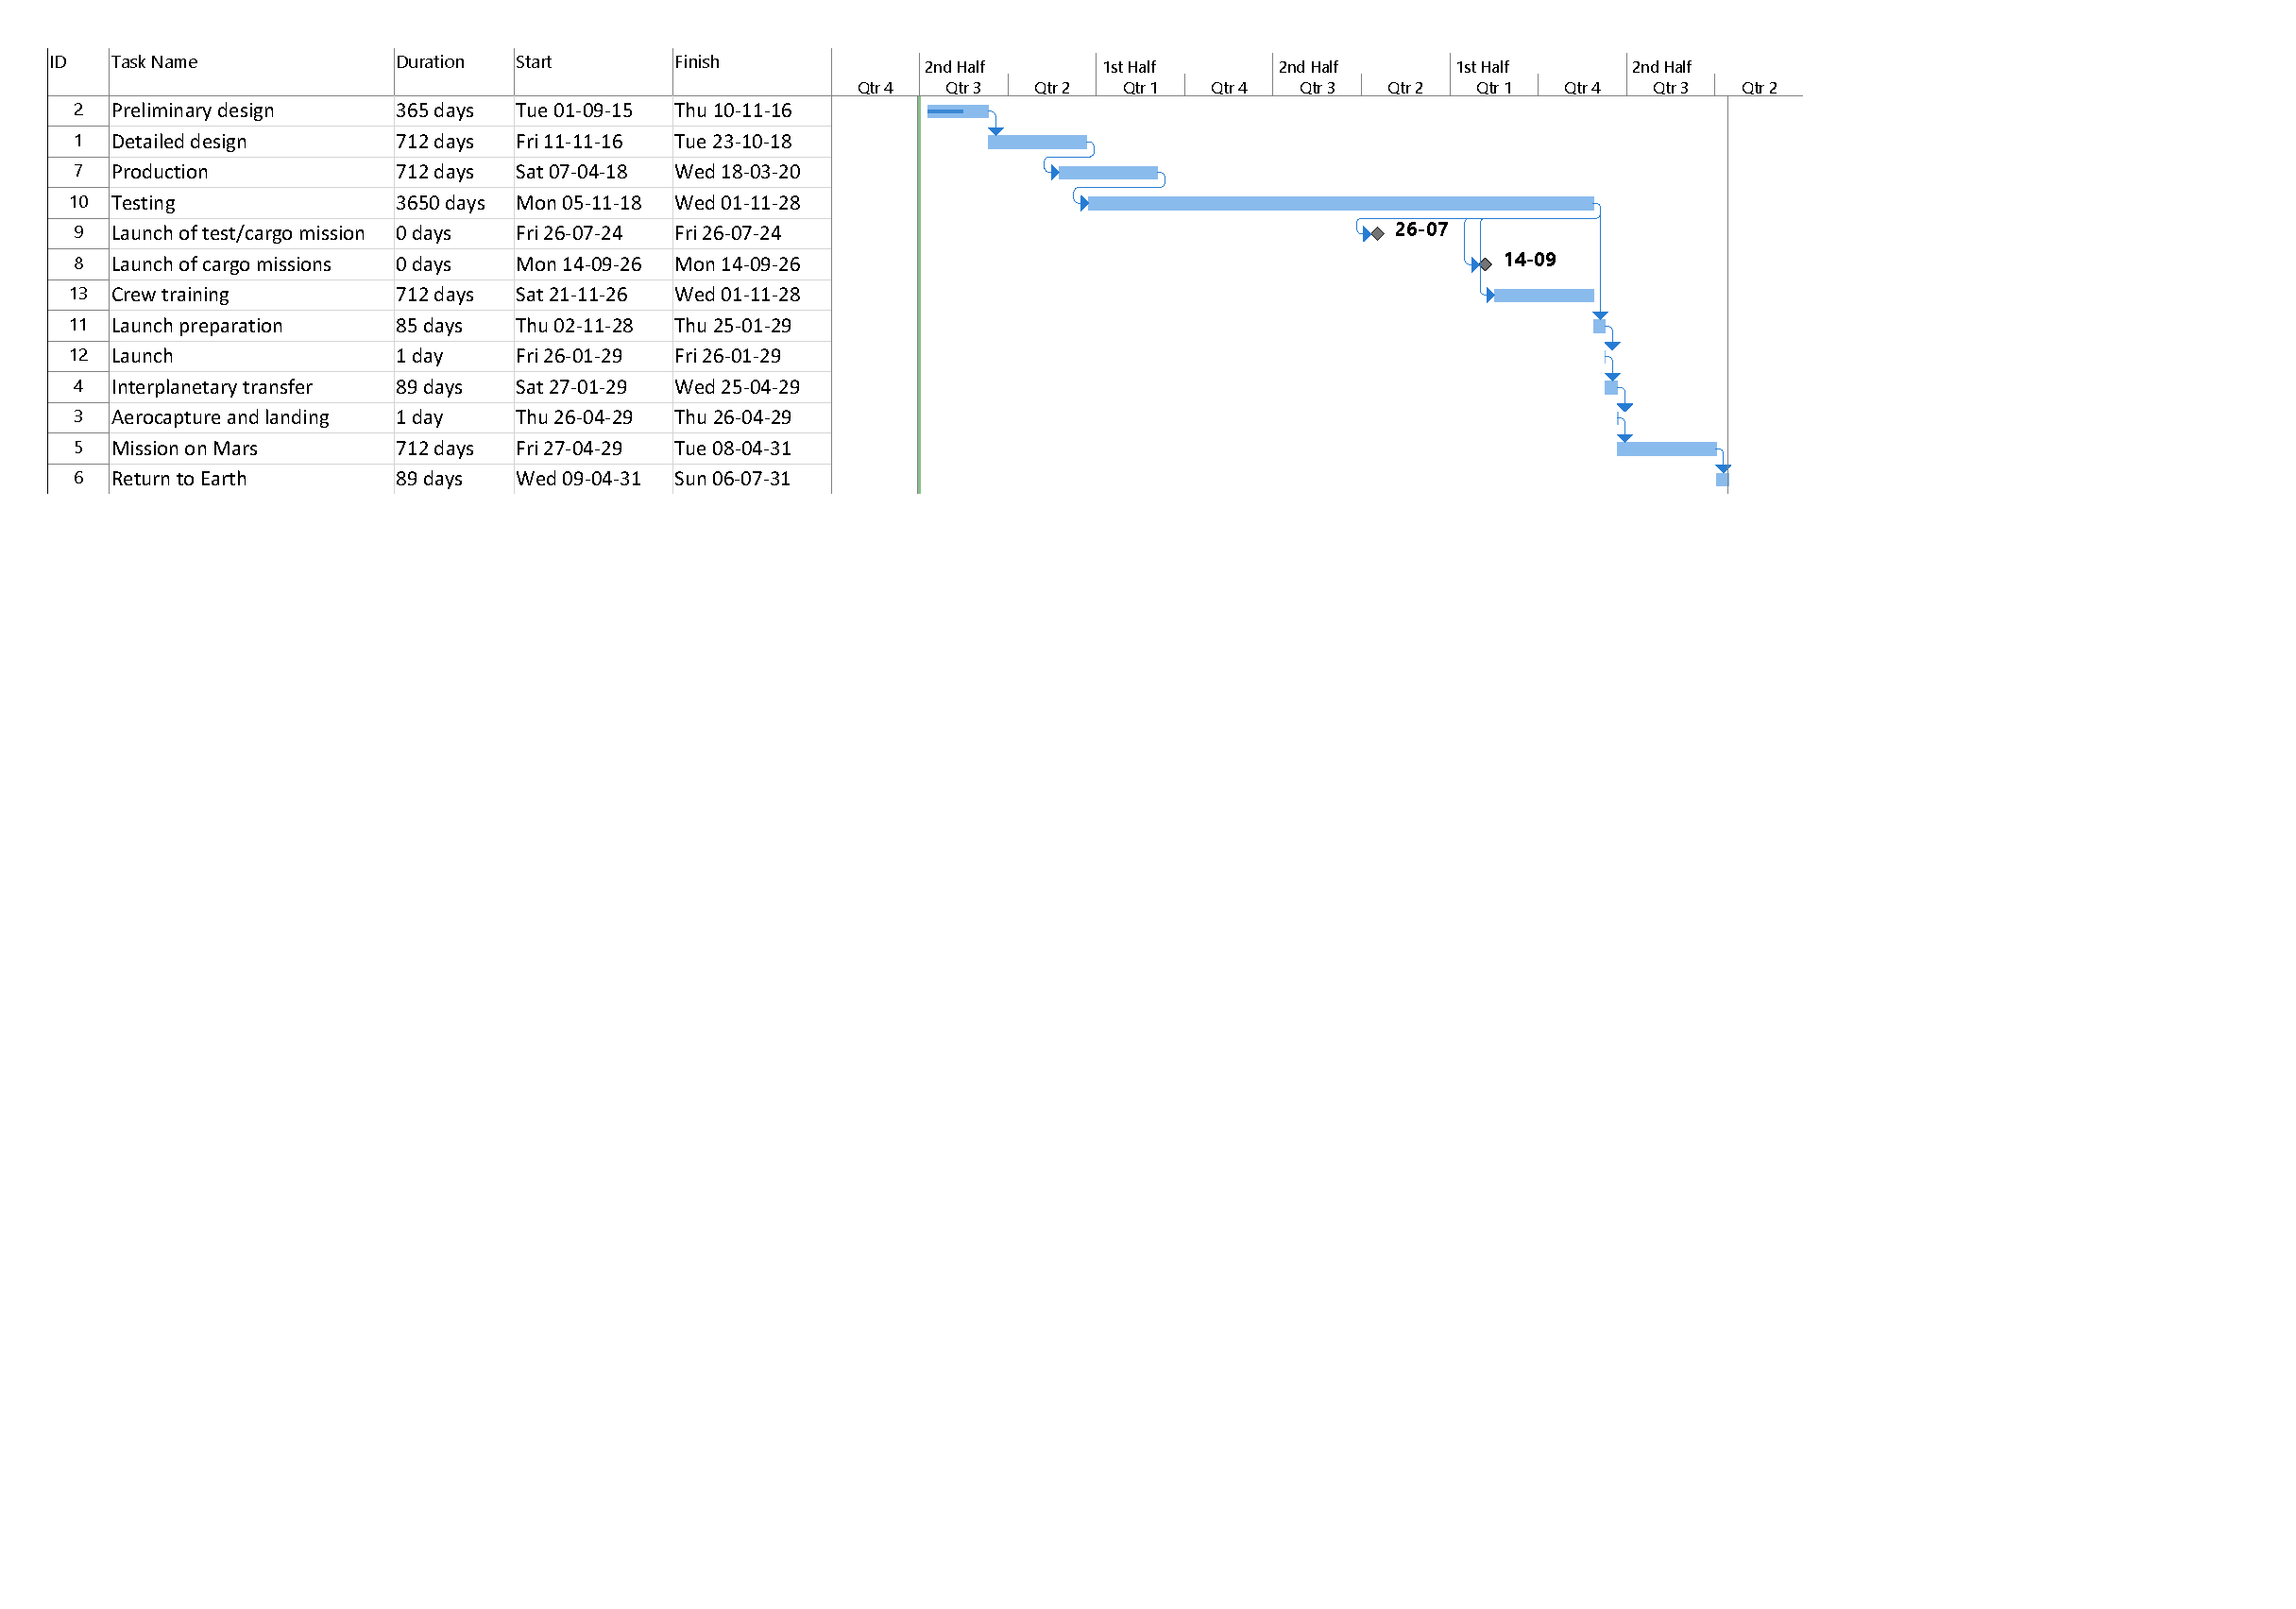
\includegraphics[width=0.98\textwidth]{./Figure/Schedule/ProjectGanttChart_v2_cropped.pdf}
	\caption{Gantt chart of future project activities}
	\label{fig:projectganttchart}
\end{figure}

Development times are based on representative missions \cite{Wertz2011}. Testing requires a considerable amount of time, due to the human-rated nature of the final spacecraft. Acceptance testing is done using a cargo mission, demonstrating the compliance of the spacecraft with the requirements on Mars. After that, potential required cargo missions are flown, including the \gls{erv}.

\subsubsection{Future design activities}
The crew module is to be designed. This involves the subsystems as defined in Chapter \ref{ch:crewmod}, the crew cabin lay-out and the packaging of the subsystems as outlined in Section \ref{sec:crewpackaging}. Moreover, the decelerator requires further detailed design to fully establish its configuration and ready it for production and integration. 

\subsubsection{Testing activities} \label{sec:TestAct}
Table \ref{tab:tests} gives an overview of proposed testing activities. In addition, it outlines the articles on which these are performed and the purpose of the tests.

\begin{table}
	\caption{An overview of proposed testing activities}
	\label{tab:tests}
	\hspace{-5mm}
	\begin{tabular}{|p{3.5cm}|p{4.5cm}|p{7cm}|}
		\hline
		\multicolumn{1}{|c|}{\textbf{Testing activity}}
		&
		\multicolumn{1}{c|}{\textbf{Performed on}}
		&
		\multicolumn{1}{c|}{\textbf{Purpose}}
		\\\hline\hline
		\begin{tabular}{p{3.3cm}}Wind tunnel testing\end{tabular}
		&
		\begin{tabular}{p{4.3cm}}Scaled decelerator wind tunnel\end{tabular}
		&
		\begin{tabular}{p{6.8cm}}1) Estimate aerodynamic properties\\ 2) Investigate effect of structure flexibility\\ 3) Investigate aerodynamic phenomena \\(e.g. aero-elasticity)\end{tabular}
		\\\hline
		\begin{tabular}{p{3.3cm}}Aero-thermal testing\end{tabular}
		&
		\begin{tabular}{p{4.3cm}}- \gls{tps} lay-up samples\\ - Decelerator assembly \\ - Crew module\end{tabular}
		&
		\begin{tabular}{p{6.8cm}}1) Demonstrate heat-carrying capability \\ and temperature\\ 2) Internal heat transfer \\ (e.g. to structural layers and inflation\end{tabular}
		\\\hline
		\begin{tabular}{p{3.3cm}}Structural testing\end{tabular}
		&
		\begin{tabular}{p{4.3cm}}- PBO Zylon\textsuperscript{\textregistered} samples\\ - Decelerator assembly\\ - Crew module\end{tabular}
		&
		\begin{tabular}{p{6.8cm}}1) Demonstrate load-carrying capability\\ 2) Investigate decelerator deflection\\ 3) Estimate effect of temperature on \\mechanical properties\\ 4) Determine effect of (launch) vibrations\end{tabular}
		\\\hline
		\begin{tabular}{p{3.3cm}}Deployment system testing\end{tabular}
		&
		\begin{tabular}{p{4.3cm}}- Strap-band assembly\\ - Centre body release\\ - Decelerator assembly\end{tabular}
		&
		\begin{tabular}{p{6.8cm}}Investigate reliability of deployment\end{tabular}
		\\\hline
		\begin{tabular}{p{3.3cm}}End-to-End information system testing\end{tabular}
		&
		\begin{tabular}{p{4.3cm}}Avionics (\gls{cdh}, \gls{adcs} and telecommunications)\end{tabular}
		&
		\begin{tabular}{p{6.8cm}}Ascertain compatibility of data handling systems\end{tabular}
		\\\hline
		\begin{tabular}{p{3.3cm}}Flight testing (Earth)\end{tabular}
		&
		\begin{tabular}{p{4.3cm}}Prototype scaled-down model (unmanned)\end{tabular}
		&
		\begin{tabular}{p{6.8cm}}1) Determine control system performance\\ 2) Determine scaled-down vehicle performance\\ 3) Validate analysis models\end{tabular}
		\\\hline
		\begin{tabular}{p{3.3cm}}Flight testing (Earth)\end{tabular}
		&
		\begin{tabular}{p{4.3cm}}Prototype full-scale model (unmanned)\end{tabular}
		&
		\begin{tabular}{p{6.8cm}}1) Validate scalability of design\\ 2) Determine integrated vehicle performance\end{tabular}
		\\\hline
		\begin{tabular}{p{3.3cm}}Mission scenario testing (simulation)\end{tabular}
		&
		\begin{tabular}{p{4.3cm}}Avionics (\gls{cdh}, \gls{adcs} and telecommunications)\end{tabular}
		&
		\begin{tabular}{p{6.8cm}}Demonstrate that flight hardware and software can execute the mission in terms of data flow with no time constraints\end{tabular}
		\\\hline
		\begin{tabular}{p{3.3cm}}Operations readiness testing (simulation)\end{tabular}
		&
		\begin{tabular}{p{4.3cm}}Avionics (\gls{cdh}, \gls{adcs} and telecommunications)\end{tabular}
		&
		\begin{tabular}{p{6.8cm}}Demonstrate that flight hardware and software can execute the mission in terms of data flow with real timeline\end{tabular}
		\\\hline
		\begin{tabular}{p{3.3cm}}Acceptance testing (Mars)\end{tabular}
		&
		\begin{tabular}{p{4.3cm}}Flight full-scale model (unmanned)\end{tabular}
		&
		\begin{tabular}{p{6.8cm}}Demonstrate system performance under limit loads\end{tabular}
		\\\hline
		\begin{tabular}{p{3.3cm}}Pilot training (simulation)\end{tabular}
		&
		\begin{tabular}{p{4.3cm}}Crew members\end{tabular}
		&
		\begin{tabular}{p{6.8cm}}Investigate man-machine interaction during interplanetary flight and entry\end{tabular}
		\\\hline
	\end{tabular}
\end{table}


\subsubsection{Production and integration}
Production and integration of the vehicle commences by a definition and analysis of the most cost-effective manufacturing methods and the most reliable and cost-effective joining methods. Hereafter, production and integration proceed in dedicated facilities with a dedicated work crew to take full advantage of crew experience and learning effect. In view of sustainability, non-value-adding activities are to be minimised in conformance with the lean manufacturing principle. 

\subsubsection{Crew preparation}
Crew members are to be trained and prepared for the 89-day journey and ensuing entry, during which they are exposed to high g-loads. Selection, training and preparation of crew members shall include their physical fitness, capability to perform required on-board activities and mental state for their isolatory condition.

\subsubsection{Establishment of a Martian infrastructure}
It is proposed that the entry vehicle is first flown unmanned, in the acceptance testing, to Mars to carry cargo required to establish an infrastructure. In addition, an infrastructure shall be laid out on Mars by previous missions. To this end, the required facilities on Mars are to be inventoried, packaged and sent as cargo on these missions.



